\section{Capítulo 8 -- Caracteres e strings}

Boa parte dos dados que um programa manipula é texto: nomes, endereços, e-mails, senhas, mensagens, o conteúdo de um documento. Até aqui, os textos só apareceram como mensagens fixas no \texttt{cout}. Neste capítulo, eles passam a ser dados de verdade: você vai ver como o computador representa cada caractere como um número, como guardar e ler textos com o tipo \texttt{string}, como percorrê-los letra por letra, como procurar, recortar e substituir pedaços, e por que as letras acentuadas do português exigem um cuidado especial. No fim, tudo se junta em um programa que cifra mensagens.

\subsection{8.1 Caracteres são números}

O tipo \texttt{char} guarda \textbf{um} caractere, escrito entre \textbf{aspas simples}: \texttt{\textquotesingle{}A\textquotesingle{}}, \texttt{\textquotesingle{}7\textquotesingle{}}, \texttt{\textquotesingle{} \textquotesingle{}}. Por dentro, o computador não guarda letras, só números: cada caractere tem um código, definido por uma tabela. A tabela básica, usada por praticamente todos os computadores, é a \textbf{ASCII}, que numera de 0 a 127 as letras sem acento, os dígitos, a pontuação e alguns caracteres de controle, como a quebra de linha.

\begin{center}
\begin{tabular}{@{}p{0.34\linewidth}p{0.24\linewidth}p{0.26\linewidth}@{}}
\toprule
\rowcolor{headergray}
\tblheader{Caracteres} & \tblheader{Códigos} & \tblheader{Exemplo} \\
\midrule
espaço & 32 & \texttt{\textquotesingle{} \textquotesingle{}} = 32 \\
\rowcolor{rowgray} dígitos \texttt{\textquotesingle{}0\textquotesingle{}} a \texttt{\textquotesingle{}9\textquotesingle{}} & 48 a 57 & \texttt{\textquotesingle{}7\textquotesingle{}} = 55 \\
maiúsculas \texttt{\textquotesingle{}A\textquotesingle{}} a \texttt{\textquotesingle{}Z\textquotesingle{}} & 65 a 90 & \texttt{\textquotesingle{}C\textquotesingle{}} = 67 \\
\rowcolor{rowgray} minúsculas \texttt{\textquotesingle{}a\textquotesingle{}} a \texttt{\textquotesingle{}z\textquotesingle{}} & 97 a 122 & \texttt{\textquotesingle{}c\textquotesingle{}} = 99 \\
\bottomrule
\end{tabular}
\end{center}

Não é preciso decorar os números, mas vale entender a organização: os dígitos, as maiúsculas e as minúsculas vêm \textbf{em sequência}, e cada minúscula fica exatamente 32 posições depois da maiúscula correspondente. Como um \texttt{char} é um número pequeno, dá para fazer contas com ele:

\begin{codigo}
\begin{Verbatim}[breaklines=true, breaksymbolleft={}, fontsize=\footnotesize]
#include <iostream>
using namespace std;

int main() {
    char letra = 'A';
    cout << letra << " tem código " << int(letra) << endl;  // 65
    char proxima = letra + 1;
    cout << proxima << endl;                // B
    char digito = '7';
    int valor = digito - '0';               // 55 - 48 = 7
    cout << valor * 2 << endl;              // 14
    cout << char('g' - 'a' + 'A') << endl;  // G
    return 0;
}
\end{Verbatim}
\end{codigo}

Dois truques aparecem aí e vão ser usados no capítulo inteiro. \texttt{digito - \textquotesingle{}0\textquotesingle{}} transforma o caractere de um dígito no número que ele representa, porque os dígitos são consecutivos a partir do \texttt{\textquotesingle{}0\textquotesingle{}}. E \texttt{c - \textquotesingle{}a\textquotesingle{}} dá a posição de uma minúscula no alfabeto (\texttt{\textquotesingle{}a\textquotesingle{}} é 0, \texttt{\textquotesingle{}b\textquotesingle{}} é 1\ldots), que somada a \texttt{\textquotesingle{}A\textquotesingle{}} dá a maiúscula correspondente.

No Portugol do VisuAlg não existe um tipo para um único caractere: o tipo \texttt{caractere} guarda textos de qualquer tamanho. As funções \texttt{asc("A")}, que devolve 65, e \texttt{carac(65)}, que devolve \texttt{"A"}, fazem a conversão entre caracteres e códigos.

\subsection{8.2 O tipo string}

Uma \textbf{string} é uma sequência de caracteres. Em C++, ela é o tipo \texttt{string}, da biblioteca \texttt{<string>}, e seus valores literais são escritos entre \textbf{aspas duplas}. Uma string se parece muito com o \texttt{vector} do Capítulo 7: cada caractere tem um índice, a partir de 0, e o tamanho é dado por \texttt{size()} (ou pelo sinônimo \texttt{length()}).

\begin{center}
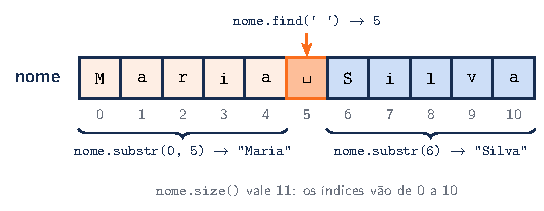
\includegraphics[width=0.85\linewidth,keepaspectratio]{imagens/capitulo-08_string.pdf}
\end{center}

\begin{codigo}
\begin{Verbatim}[breaklines=true, breaksymbolleft={}, fontsize=\footnotesize]
#include <iostream>
#include <string>
using namespace std;

int main() {
    string nome = "Ada";
    string sobrenome = "Lovelace";
    string completo = nome + " " + sobrenome;   // concatenação
    cout << completo << endl;                   // Ada Lovelace
    cout << completo.size() << " caracteres" << endl;   // 12
    cout << completo[0] << completo[4] << endl; // AL
    completo[0] = 'a';                          // pode alterar
    cout << completo << endl;                   // ada Lovelace
    completo += "!";                            // acrescenta
    cout << completo << endl;                   // ada Lovelace!
    return 0;
}
\end{Verbatim}
\end{codigo}

O operador \texttt{+} junta (\textbf{concatena}) duas strings, e \texttt{+=} acrescenta no fim. As strings também podem ser comparadas com \texttt{==}, \texttt{!=}, \texttt{<} e os demais operadores relacionais. A comparação é feita caractere a caractere, pelos códigos, como na ordem de um dicionário: \texttt{"casa" < "caso"}, porque na primeira diferença \texttt{\textquotesingle{}a\textquotesingle{}} vem antes de \texttt{\textquotesingle{}o\textquotesingle{}}. Mas, como a ordem é a dos códigos, toda maiúscula vem antes de qualquer minúscula, e \texttt{"Zebra" < "abacate"} é verdadeiro. Para comparar sem diferenciar maiúsculas de minúsculas, converta as duas strings para a mesma forma antes (Seção 8.4).

No Portugol, o tipo é \texttt{caractere}, a concatenação também é feita com \texttt{+}, e as operações são funções:

\begin{codigo}
\begin{Verbatim}[breaklines=true, breaksymbolleft={}, fontsize=\footnotesize]
algoritmo "Textos"
var
   nome: caractere
inicio
   escreva("Nome: ")
   leia(nome)
   escreval("Tamanho: ", compr(nome))
   escreval("Primeira letra: ", copia(nome, 1, 1))
   escreval("Em maiúsculas: ", maiusc(nome))
   escreval("Olá, " + nome + "!")
fimalgoritmo
\end{Verbatim}
\end{codigo}

No Portugol, as posições começam em 1: \texttt{copia(nome, 1, 1)} copia, a partir da posição 1, um caractere.

\subsection{8.3 Lendo textos}

O \texttt{cin >>} lê uma \textbf{palavra}: ele para no primeiro espaço. Com a entrada \texttt{Ada Lovelace}, \texttt{cin >> nome} guarda só \texttt{"Ada"}, e o \texttt{"Lovelace"} fica esperando a próxima leitura. Para ler uma linha inteira, com espaços, use \texttt{getline(cin, nome)}.

Misturar os dois exige um cuidado. Quando o usuário digita a idade e tecla Enter, o \texttt{cin >> idade} lê o número e deixa o Enter para trás. Um \texttt{getline} logo depois encontra esse Enter e devolve uma linha vazia, sem esperar o usuário. A solução é descartar os espaços e quebras de linha pendentes com \texttt{ws} antes do \texttt{getline}:

\begin{codigo}
\begin{Verbatim}[breaklines=true, breaksymbolleft={}, fontsize=\footnotesize]
#include <iostream>
#include <string>
using namespace std;

int main() {
    int idade;
    string nome;
    cout << "Idade: ";
    cin >> idade;
    cout << "Nome completo: ";
    getline(cin >> ws, nome);    // ws descarta o Enter que sobrou
    cout << nome << ", " << idade << " anos" << endl;
    return 0;
}
// Entrada: 36, depois Ada Lovelace  ->  Ada Lovelace, 36 anos
\end{Verbatim}
\end{codigo}

\subsection{8.4 Percorrendo uma string}

Como uma string é uma sequência, um laço pode visitar cada caractere. Além do \texttt{for} com índice, o C++ tem uma forma mais curta para percorrer uma sequência inteira, o \textbf{for de intervalo}: \texttt{for (char c : texto)} executa o bloco uma vez para cada caractere, guardado em \texttt{c}. Se a variável for uma referência, \texttt{for (char \&c : texto)}, alterar \texttt{c} altera a própria string, exatamente como na passagem por referência do Capítulo 6.

A biblioteca \texttt{<cctype>} tem funções para classificar e converter caracteres: \texttt{isalpha} (é letra?), \texttt{isdigit} (é dígito?), \texttt{isspace} (é espaço?), \texttt{isalnum} (é letra ou dígito?), \texttt{toupper} e \texttt{tolower} (convertem para maiúscula e minúscula). O programa abaixo usa várias delas:

\begin{codigo}
\begin{Verbatim}[breaklines=true, breaksymbolleft={}, fontsize=\footnotesize]
#include <iostream>
#include <string>
#include <cctype>      // isdigit, isspace, toupper, tolower...
using namespace std;

bool ehVogal(unsigned char c) {
    c = tolower(c);
    return c == 'a' || c == 'e' || c == 'i' || c == 'o'
        || c == 'u';
}

int main() {
    string frase;
    cout << "Frase: ";
    getline(cin, frase);
    int vogais = 0, digitos = 0, espacos = 0;
    for (unsigned char c : frase) {         // cada caractere
        if (ehVogal(c)) vogais++;
        else if (isdigit(c)) digitos++;
        else if (isspace(c)) espacos++;
    }
    cout << vogais << " vogais, " << digitos << " dígitos, "
         << espacos << " espaços" << endl;
    for (char &c : frase) {                 // & altera a frase
        c = toupper((unsigned char) c);
    }
    cout << frase << endl;
    return 0;
}
// Entrada: Turma 2026 da noite
// Saída:   6 vogais, 4 dígitos, 3 espaços
//          TURMA 2026 DA NOITE
\end{Verbatim}
\end{codigo}

O \texttt{unsigned char} parece um detalhe estranho, mas tem motivo: as funções de \texttt{<cctype>} exigem um código entre 0 e 255, e um \texttt{char} comum pode ser negativo para os caracteres fora da tabela ASCII, como os acentuados (Seção 8.7). Converter para \texttt{unsigned char} antes de chamá-las evita o problema.

\subsection{8.5 Procurando, recortando e convertendo}

A classe \texttt{string} oferece operações para trabalhar com pedaços do texto. As duas mais usadas andam juntas: \texttt{find} procura um caractere ou um trecho e devolve a posição da primeira ocorrência, e \texttt{substr(p, n)} copia \texttt{n} caracteres a partir da posição \texttt{p} (sem o \texttt{n}, copia até o fim). A figura da Seção 8.2 mostra as duas em ação sobre \texttt{"Maria Silva"}.

Quando o \texttt{find} não encontra nada, ele devolve o valor especial \texttt{string::npos}. Esse valor precisa \textbf{sempre} ser testado antes de usar a posição, porque ele é um número enorme, e usá-lo como índice leva a erro.

\begin{codigo}
\begin{Verbatim}[breaklines=true, breaksymbolleft={}, fontsize=\footnotesize]
#include <iostream>
#include <string>
using namespace std;

int main() {
    string nome = "Maria Silva";
    size_t espaco = nome.find(' ');               // 5
    if (espaco != string::npos) {
        cout << nome.substr(0, espaco) << endl;   // Maria
        cout << nome.substr(espaco + 1) << endl;  // Silva
    }

    string data = "25/12/2026";
    int dia = stoi(data.substr(0, 2));            // texto -> int
    int mes = stoi(data.substr(3, 2));
    int ano = stoi(data.substr(6));
    cout << dia + mes + ano << endl;              // 2063

    string aviso = "Nota final: X";
    aviso.replace(aviso.find('X'), 1, to_string(9));
    cout << aviso << endl;                        // Nota final: 9
    return 0;
}
\end{Verbatim}
\end{codigo}

As funções \texttt{stoi} (\textit{string to int}) e \texttt{stod} (\textit{string to double}) convertem um texto em número, e \texttt{to\_string} faz o caminho contrário. A soma \texttt{dia + mes + ano} só está ali para mostrar que, depois do \texttt{stoi}, os pedaços da data são números de verdade. A tabela resume as operações mais úteis, com os equivalentes do Portugol:

\begin{center}
\begin{tabular}{@{}p{0.27\linewidth}p{0.36\linewidth}p{0.25\linewidth}@{}}
\toprule
\rowcolor{headergray}
\tblheader{C++} & \tblheader{O que faz} & \tblheader{Portugol} \\
\midrule
\texttt{s.size()} & tamanho & \texttt{compr(s)} \\
\rowcolor{rowgray} \texttt{s + t} & concatena & \texttt{s + t} \\
\texttt{s.substr(p, n)} & \texttt{n} caracteres a partir de \texttt{p} & \texttt{copia(s, p, n)} \\
\rowcolor{rowgray} \texttt{s.find(t)} & posição de \texttt{t} em \texttt{s} & \texttt{pos(t, s)} \\
\texttt{s.insert(p, t)} & insere \texttt{t} na posição \texttt{p} & -- \\
\rowcolor{rowgray} \texttt{s.erase(p, n)} & apaga \texttt{n} caracteres & -- \\
\texttt{s.replace(p, n, t)} & troca \texttt{n} caracteres por \texttt{t} & -- \\
\rowcolor{rowgray} \texttt{toupper(c)} & maiúscula (um caractere) & \texttt{maiusc(s)} \\
\texttt{stoi(s)}, \texttt{stod(s)} & texto para número & \texttt{caracpnum(s)} \\
\rowcolor{rowgray} \texttt{to\_string(x)} & número para texto & \texttt{numpcarac(x)} \\
\bottomrule
\end{tabular}
\end{center}

Lembre que no Portugol as posições começam em 1, e que \texttt{pos} devolve 0 quando não encontra o trecho. O \texttt{maiusc} do Portugol converte a string inteira, enquanto o \texttt{toupper} do C++ converte um caractere por vez.

\subsection{8.6 Algoritmos com strings: palíndromos}

Um \textbf{palíndromo} é um texto que se lê igual nos dois sentidos, como ``radar'' ou ``Roma me tem amor''. Para frases, a convenção é ignorar espaços, pontuação e a diferença entre maiúsculas e minúsculas. O algoritmo tem duas etapas: primeiro, monta uma versão ``limpa'' do texto, só com letras e dígitos em minúsculas; depois, compara o primeiro caractere com o último, o segundo com o penúltimo, e assim por diante, com os dois índices que caminham um em direção ao outro, como na inversão de vetores do Capítulo 7.

\begin{codigo}
\begin{Verbatim}[breaklines=true, breaksymbolleft={}, fontsize=\footnotesize]
#include <iostream>
#include <string>
#include <cctype>
using namespace std;

bool ehPalindromo(const string &texto) {
    string limpo;
    for (unsigned char c : texto) {
        if (isalnum(c)) limpo += char(tolower(c));
    }
    int i = 0, j = int(limpo.size()) - 1;
    while (i < j) {
        if (limpo[i] != limpo[j]) return false;  // diferença
        i++;
        j--;
    }
    return true;
}

int main() {
    string frases[] = {"radar", "Roma me tem amor",
                       "A base do teto desaba", "algoritmo"};
    for (const string &f : frases) {
        cout << f << ": " << (ehPalindromo(f) ? "sim" : "não")
             << endl;
    }
    return 0;
}
// radar: sim   Roma me tem amor: sim
// A base do teto desaba: sim   algoritmo: não
\end{Verbatim}
\end{codigo}

O \texttt{return false} encerra a busca na primeira diferença: não adianta continuar comparando. A função recebe o texto por referência constante (Capítulo 6), porque só precisa lê-lo. E o \texttt{for} de intervalo também funciona com vetores, como o \texttt{frases} do \texttt{main}.

\subsection{8.7 Acentos e a codificação UTF-8}

A tabela ASCII não tem letras acentuadas. Para representar os caracteres de todas as línguas, o padrão atual é o \textbf{Unicode}, e a forma mais comum de gravá-lo é a codificação \textbf{UTF-8}. Nela, os caracteres da tabela ASCII continuam ocupando um byte, mas os demais ocupam dois ou mais. Como o \texttt{string} do C++ é uma sequência de bytes, e não de letras, isso tem consequências para quem escreve em português:

\begin{codigo}
\begin{Verbatim}[breaklines=true, breaksymbolleft={}, fontsize=\footnotesize]
#include <iostream>
#include <string>
using namespace std;

int main() {
    string palavra = "ação";
    cout << palavra.size() << endl;   // 6, e não 4
    return 0;                         // (ç e ã têm 2 bytes)
}
\end{Verbatim}
\end{codigo}

Por isso, \texttt{palavra[1]} não é o \texttt{\textquotesingle{}ç\textquotesingle{}}, mas só o primeiro dos seus dois bytes, e \texttt{toupper} não transforma \texttt{\textquotesingle{}ã\textquotesingle{}} em \texttt{\textquotesingle{}Ã\textquotesingle{}}. Contar, inverter ou converter letra por letra um texto acentuado exige bibliotecas próprias para Unicode, que estão além desta disciplina. Os exemplos deste capítulo que processam caractere por caractere supõem textos sem acentos. Guardar, ler, mostrar, concatenar e comparar com \texttt{==} textos acentuados, por outro lado, funciona normalmente.

\subsection{8.8 Strings no estilo C}

Antes do tipo \texttt{string}, a linguagem C representava um texto como um \textbf{vetor de char} terminado pelo caractere especial \texttt{\textquotesingle{}\textbackslash 0\textquotesingle{}} (o caractere de código zero), que marca onde o texto acaba. Esse formato ainda aparece em código antigo, em bibliotecas e nos textos entre aspas duplas, que no C++ são, na verdade, vetores de \texttt{char}.

\begin{codigo}
\begin{Verbatim}[breaklines=true, breaksymbolleft={}, fontsize=\footnotesize]
#include <iostream>
#include <cstring>     // strlen, strcmp, strcpy
using namespace std;

int main() {
    char nome[10] = "Ana";     // 'A' 'n' 'a' '\0' e zeros
    cout << nome << " tem " << strlen(nome) << " letras" << endl;
    cout << (strcmp(nome, "Ana") == 0) << endl;   // 1: iguais
    return 0;
}
\end{Verbatim}
\end{codigo}

As strings do estilo C herdam todos os riscos dos vetores: têm capacidade fixa, não podem ser comparadas com \texttt{==} (que compara endereços, e não o conteúdo; para isso existe \texttt{strcmp}) nem atribuídas com \texttt{=}, e é fácil escrever além do fim. Em programas novos, prefira sempre o \texttt{string}.

\subsection{8.9 Um programa completo: a cifra de César}

Um dos métodos de criptografia mais antigos que se conhecem é atribuído a Júlio César, que o usava em mensagens militares: cada letra é trocada pela letra que fica um número fixo de posições adiante no alfabeto, a \textbf{chave}. Com chave 3, o A vira D, o B vira E e, ao chegar ao fim, o alfabeto recomeça: o X vira A.

\begin{center}
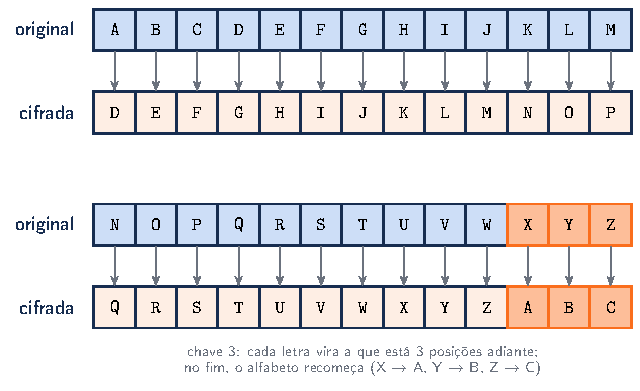
\includegraphics[width=0.7\linewidth,keepaspectratio]{imagens/capitulo-08_cesar.pdf}
\end{center}

A conta usa os dois truques da Seção 8.1. A posição da letra no alfabeto é \texttt{c - \textquotesingle{}a\textquotesingle{}}; somando a chave e tirando o resto da divisão por 26, a posição ``dá a volta'' no fim do alfabeto; e somar \texttt{\textquotesingle{}a\textquotesingle{}} de novo transforma a posição em letra. Para decifrar, basta cifrar de novo com a chave \texttt{26 - k}, que completa a volta.

\begin{codigo}
\begin{Verbatim}[breaklines=true, breaksymbolleft={}, fontsize=\footnotesize]
#include <iostream>
#include <string>
using namespace std;

char deslocar(char c, int k) {
    k = (k % 26 + 26) % 26;          // chave entre 0 e 25
    if (c >= 'a' && c <= 'z') return 'a' + (c - 'a' + k) % 26;
    if (c >= 'A' && c <= 'Z') return 'A' + (c - 'A' + k) % 26;
    return c;                        // o resto não muda
}

string cifrar(const string &texto, int k) {
    string resultado = texto;
    for (char &c : resultado) c = deslocar(c, k);
    return resultado;
}

int main() {
    int chave;
    string mensagem;
    cout << "Chave: ";
    cin >> chave;
    cout << "Mensagem: ";
    getline(cin >> ws, mensagem);
    string secreta = cifrar(mensagem, chave);
    cout << "Cifrada:   " << secreta << endl;
    cout << "Decifrada: " << cifrar(secreta, 26 - chave) << endl;
    return 0;
}
// Chave 3, "Ataque ao amanhecer"
// Cifrada:   Dwdtxh dr dpdqkhfhu
// Decifrada: Ataque ao amanhecer
\end{Verbatim}
\end{codigo}

A primeira linha de \texttt{deslocar} traz qualquer chave, inclusive negativa ou maior que 26, para a faixa de 0 a 25. Sem ela, uma chave negativa daria um resto negativo e um caractere fora do alfabeto. Os caracteres que não são letras, como espaços e pontuação, passam sem alteração.

A cifra de César é ótima para praticar strings, mas péssima para proteger segredos: como só existem 25 chaves possíveis, basta testar todas para ler a mensagem. A criptografia usada hoje, nos sites e aplicativos, se baseia em matemática bem mais sofisticada.

\subsection{Erros Comuns}

\begin{itemize}
  \item \textbf{Confundir aspas simples e duplas.} \texttt{\textquotesingle{}A\textquotesingle{}} é um \texttt{char}; \texttt{"A"} é um texto. \texttt{\textquotesingle{}Ana\textquotesingle{}} não é válido.
  \item \textbf{Usar \texttt{getline} logo depois de \texttt{cin >>}.} O Enter que sobrou é lido como uma linha vazia. Use \texttt{getline(cin >> ws, s)}.
  \item \textbf{Ler um nome com espaços usando \texttt{cin >>}.} Só a primeira palavra é lida.
  \item \textbf{Usar a posição do \texttt{find} sem testar \texttt{npos}.} Quando o trecho não existe, a posição é um número enorme e inválido.
  \item \textbf{Acessar \texttt{s[i]} fora do tamanho.} Como nos vetores, \texttt{s[s.size()]} não é um caractere válido do texto.
  \item \textbf{Esquecer que a comparação diferencia maiúsculas.} \texttt{"ana" == "Ana"} é falso, e \texttt{"Zebra" < "abacate"} é verdadeiro.
  \item \textbf{Confundir o caractere de um dígito com o número.} \texttt{\textquotesingle{}7\textquotesingle{}} vale 55; o número 7 é \texttt{\textquotesingle{}7\textquotesingle{} - \textquotesingle{}0\textquotesingle{}}.
  \item \textbf{Processar letra por letra um texto com acentos.} Em UTF-8, uma letra acentuada ocupa mais de um byte.
  \item \textbf{Comparar strings do estilo C com \texttt{==}.} Use \texttt{strcmp}, ou melhor, use \texttt{string}.
\end{itemize}
